% Options for packages loaded elsewhere
\PassOptionsToPackage{unicode}{hyperref}
\PassOptionsToPackage{hyphens}{url}
\PassOptionsToPackage{dvipsnames,svgnames,x11names}{xcolor}
%
\documentclass[
  b5paper,
  xelatex, ja=standard]{bxjsbook}

\usepackage{amsmath,amssymb}
\usepackage{iftex}
\ifPDFTeX
  \usepackage[T1]{fontenc}
  \usepackage[utf8]{inputenc}
  \usepackage{textcomp} % provide euro and other symbols
\else % if luatex or xetex
  \usepackage{unicode-math}
  \defaultfontfeatures{Scale=MatchLowercase}
  \defaultfontfeatures[\rmfamily]{Ligatures=TeX,Scale=1}
\fi
\usepackage{lmodern}
\ifPDFTeX\else  
    % xetex/luatex font selection
\fi
% Use upquote if available, for straight quotes in verbatim environments
\IfFileExists{upquote.sty}{\usepackage{upquote}}{}
\IfFileExists{microtype.sty}{% use microtype if available
  \usepackage[]{microtype}
  \UseMicrotypeSet[protrusion]{basicmath} % disable protrusion for tt fonts
}{}
\makeatletter
\@ifundefined{KOMAClassName}{% if non-KOMA class
  \IfFileExists{parskip.sty}{%
    \usepackage{parskip}
  }{% else
    \setlength{\parindent}{0pt}
    \setlength{\parskip}{6pt plus 2pt minus 1pt}}
}{% if KOMA class
  \KOMAoptions{parskip=half}}
\makeatother
\usepackage{xcolor}
\setlength{\emergencystretch}{3em} % prevent overfull lines
\setcounter{secnumdepth}{5}
% Make \paragraph and \subparagraph free-standing
\ifx\paragraph\undefined\else
  \let\oldparagraph\paragraph
  \renewcommand{\paragraph}[1]{\oldparagraph{#1}\mbox{}}
\fi
\ifx\subparagraph\undefined\else
  \let\oldsubparagraph\subparagraph
  \renewcommand{\subparagraph}[1]{\oldsubparagraph{#1}\mbox{}}
\fi

\usepackage{color}
\usepackage{fancyvrb}
\newcommand{\VerbBar}{|}
\newcommand{\VERB}{\Verb[commandchars=\\\{\}]}
\DefineVerbatimEnvironment{Highlighting}{Verbatim}{commandchars=\\\{\}}
% Add ',fontsize=\small' for more characters per line
\usepackage{framed}
\definecolor{shadecolor}{RGB}{241,243,245}
\newenvironment{Shaded}{\begin{snugshade}}{\end{snugshade}}
\newcommand{\AlertTok}[1]{\textcolor[rgb]{0.68,0.00,0.00}{#1}}
\newcommand{\AnnotationTok}[1]{\textcolor[rgb]{0.37,0.37,0.37}{#1}}
\newcommand{\AttributeTok}[1]{\textcolor[rgb]{0.40,0.45,0.13}{#1}}
\newcommand{\BaseNTok}[1]{\textcolor[rgb]{0.68,0.00,0.00}{#1}}
\newcommand{\BuiltInTok}[1]{\textcolor[rgb]{0.00,0.23,0.31}{#1}}
\newcommand{\CharTok}[1]{\textcolor[rgb]{0.13,0.47,0.30}{#1}}
\newcommand{\CommentTok}[1]{\textcolor[rgb]{0.37,0.37,0.37}{#1}}
\newcommand{\CommentVarTok}[1]{\textcolor[rgb]{0.37,0.37,0.37}{\textit{#1}}}
\newcommand{\ConstantTok}[1]{\textcolor[rgb]{0.56,0.35,0.01}{#1}}
\newcommand{\ControlFlowTok}[1]{\textcolor[rgb]{0.00,0.23,0.31}{#1}}
\newcommand{\DataTypeTok}[1]{\textcolor[rgb]{0.68,0.00,0.00}{#1}}
\newcommand{\DecValTok}[1]{\textcolor[rgb]{0.68,0.00,0.00}{#1}}
\newcommand{\DocumentationTok}[1]{\textcolor[rgb]{0.37,0.37,0.37}{\textit{#1}}}
\newcommand{\ErrorTok}[1]{\textcolor[rgb]{0.68,0.00,0.00}{#1}}
\newcommand{\ExtensionTok}[1]{\textcolor[rgb]{0.00,0.23,0.31}{#1}}
\newcommand{\FloatTok}[1]{\textcolor[rgb]{0.68,0.00,0.00}{#1}}
\newcommand{\FunctionTok}[1]{\textcolor[rgb]{0.28,0.35,0.67}{#1}}
\newcommand{\ImportTok}[1]{\textcolor[rgb]{0.00,0.46,0.62}{#1}}
\newcommand{\InformationTok}[1]{\textcolor[rgb]{0.37,0.37,0.37}{#1}}
\newcommand{\KeywordTok}[1]{\textcolor[rgb]{0.00,0.23,0.31}{#1}}
\newcommand{\NormalTok}[1]{\textcolor[rgb]{0.00,0.23,0.31}{#1}}
\newcommand{\OperatorTok}[1]{\textcolor[rgb]{0.37,0.37,0.37}{#1}}
\newcommand{\OtherTok}[1]{\textcolor[rgb]{0.00,0.23,0.31}{#1}}
\newcommand{\PreprocessorTok}[1]{\textcolor[rgb]{0.68,0.00,0.00}{#1}}
\newcommand{\RegionMarkerTok}[1]{\textcolor[rgb]{0.00,0.23,0.31}{#1}}
\newcommand{\SpecialCharTok}[1]{\textcolor[rgb]{0.37,0.37,0.37}{#1}}
\newcommand{\SpecialStringTok}[1]{\textcolor[rgb]{0.13,0.47,0.30}{#1}}
\newcommand{\StringTok}[1]{\textcolor[rgb]{0.13,0.47,0.30}{#1}}
\newcommand{\VariableTok}[1]{\textcolor[rgb]{0.07,0.07,0.07}{#1}}
\newcommand{\VerbatimStringTok}[1]{\textcolor[rgb]{0.13,0.47,0.30}{#1}}
\newcommand{\WarningTok}[1]{\textcolor[rgb]{0.37,0.37,0.37}{\textit{#1}}}

\providecommand{\tightlist}{%
  \setlength{\itemsep}{0pt}\setlength{\parskip}{0pt}}\usepackage{longtable,booktabs,array}
\usepackage{calc} % for calculating minipage widths
% Correct order of tables after \paragraph or \subparagraph
\usepackage{etoolbox}
\makeatletter
\patchcmd\longtable{\par}{\if@noskipsec\mbox{}\fi\par}{}{}
\makeatother
% Allow footnotes in longtable head/foot
\IfFileExists{footnotehyper.sty}{\usepackage{footnotehyper}}{\usepackage{footnote}}
\makesavenoteenv{longtable}
\usepackage{graphicx}
\makeatletter
\def\maxwidth{\ifdim\Gin@nat@width>\linewidth\linewidth\else\Gin@nat@width\fi}
\def\maxheight{\ifdim\Gin@nat@height>\textheight\textheight\else\Gin@nat@height\fi}
\makeatother
% Scale images if necessary, so that they will not overflow the page
% margins by default, and it is still possible to overwrite the defaults
% using explicit options in \includegraphics[width, height, ...]{}
\setkeys{Gin}{width=\maxwidth,height=\maxheight,keepaspectratio}
% Set default figure placement to htbp
\makeatletter
\def\fps@figure{htbp}
\makeatother
% definitions for citeproc citations
\NewDocumentCommand\citeproctext{}{}
\NewDocumentCommand\citeproc{mm}{%
  \begingroup\def\citeproctext{#2}\cite{#1}\endgroup}
\makeatletter
 % allow citations to break across lines
 \let\@cite@ofmt\@firstofone
 % avoid brackets around text for \cite:
 \def\@biblabel#1{}
 \def\@cite#1#2{{#1\if@tempswa , #2\fi}}
\makeatother
\newlength{\cslhangindent}
\setlength{\cslhangindent}{1.5em}
\newlength{\csllabelwidth}
\setlength{\csllabelwidth}{3em}
\newenvironment{CSLReferences}[2] % #1 hanging-indent, #2 entry-spacing
 {\begin{list}{}{%
  \setlength{\itemindent}{0pt}
  \setlength{\leftmargin}{0pt}
  \setlength{\parsep}{0pt}
  % turn on hanging indent if param 1 is 1
  \ifodd #1
   \setlength{\leftmargin}{\cslhangindent}
   \setlength{\itemindent}{-1\cslhangindent}
  \fi
  % set entry spacing
  \setlength{\itemsep}{#2\baselineskip}}}
 {\end{list}}
\usepackage{calc}
\newcommand{\CSLBlock}[1]{\hfill\break\parbox[t]{\linewidth}{\strut\ignorespaces#1\strut}}
\newcommand{\CSLLeftMargin}[1]{\parbox[t]{\csllabelwidth}{\strut#1\strut}}
\newcommand{\CSLRightInline}[1]{\parbox[t]{\linewidth - \csllabelwidth}{\strut#1\strut}}
\newcommand{\CSLIndent}[1]{\hspace{\cslhangindent}#1}

\makeatletter
\def\emptypage@emptypage{%
    \hbox{}%
    \thispagestyle{headings}%
    \newpage%    
}%
\def\cleardoublepage{%
        \clearpage%
        \if@twoside%
            \ifodd\c@page%
                % do nothing
            \else%
                \emptypage@emptypage%
            \fi%
        \fi%
    }%
\makeatother
\usepackage{booktabs}
\usepackage{longtable}
\usepackage{array}
\usepackage{multirow}
\usepackage{wrapfig}
\usepackage{float}
\usepackage{colortbl}
\usepackage{pdflscape}
\usepackage{tabu}
\usepackage{threeparttable}
\usepackage{threeparttablex}
\usepackage[normalem]{ulem}
\usepackage{makecell}
\usepackage{xcolor}
\makeatletter
\@ifpackageloaded{tcolorbox}{}{\usepackage[skins,breakable]{tcolorbox}}
\@ifpackageloaded{fontawesome5}{}{\usepackage{fontawesome5}}
\definecolor{quarto-callout-color}{HTML}{909090}
\definecolor{quarto-callout-note-color}{HTML}{0758E5}
\definecolor{quarto-callout-important-color}{HTML}{CC1914}
\definecolor{quarto-callout-warning-color}{HTML}{EB9113}
\definecolor{quarto-callout-tip-color}{HTML}{00A047}
\definecolor{quarto-callout-caution-color}{HTML}{FC5300}
\definecolor{quarto-callout-color-frame}{HTML}{acacac}
\definecolor{quarto-callout-note-color-frame}{HTML}{4582ec}
\definecolor{quarto-callout-important-color-frame}{HTML}{d9534f}
\definecolor{quarto-callout-warning-color-frame}{HTML}{f0ad4e}
\definecolor{quarto-callout-tip-color-frame}{HTML}{02b875}
\definecolor{quarto-callout-caution-color-frame}{HTML}{fd7e14}
\makeatother
\makeatletter
\@ifpackageloaded{bookmark}{}{\usepackage{bookmark}}
\makeatother
\makeatletter
\@ifpackageloaded{caption}{}{\usepackage{caption}}
\AtBeginDocument{%
\ifdefined\contentsname
  \renewcommand*\contentsname{Table of contents}
\else
  \newcommand\contentsname{Table of contents}
\fi
\ifdefined\listfigurename
  \renewcommand*\listfigurename{List of Figures}
\else
  \newcommand\listfigurename{List of Figures}
\fi
\ifdefined\listtablename
  \renewcommand*\listtablename{List of Tables}
\else
  \newcommand\listtablename{List of Tables}
\fi
\ifdefined\figurename
  \renewcommand*\figurename{Figure}
\else
  \newcommand\figurename{Figure}
\fi
\ifdefined\tablename
  \renewcommand*\tablename{Table}
\else
  \newcommand\tablename{Table}
\fi
}
\@ifpackageloaded{float}{}{\usepackage{float}}
\floatstyle{ruled}
\@ifundefined{c@chapter}{\newfloat{codelisting}{h}{lop}}{\newfloat{codelisting}{h}{lop}[chapter]}
\floatname{codelisting}{Listing}
\newcommand*\listoflistings{\listof{codelisting}{List of Listings}}
\makeatother
\makeatletter
\makeatother
\makeatletter
\@ifpackageloaded{caption}{}{\usepackage{caption}}
\@ifpackageloaded{subcaption}{}{\usepackage{subcaption}}
\makeatother
\newcounter{quartocalloutnteno}
\newcommand{\quartocalloutnte}[1]{\refstepcounter{quartocalloutnteno}\label{#1}}
\ifLuaTeX
  \usepackage{selnolig}  % disable illegal ligatures
\fi
\usepackage{bookmark}

\IfFileExists{xurl.sty}{\usepackage{xurl}}{} % add URL line breaks if available
\urlstyle{same} % disable monospaced font for URLs
\hypersetup{
  pdftitle={技術系同人誌テンプレート},
  pdfauthor={やわらかクジラ},
  colorlinks=true,
  linkcolor={blue},
  filecolor={Maroon},
  citecolor={Blue},
  urlcolor={Blue},
  pdfcreator={LaTeX via pandoc}}

\title{技術系同人誌テンプレート}
\author{やわらかクジラ}
\date{2024-03-28}

\begin{document}
\maketitle

\renewcommand*\contentsname{目次}
{
\hypersetup{linkcolor=}
\setcounter{tocdepth}{2}
\tableofcontents
}
\bookmarksetup{startatroot}

\chapter*{はじめに}\label{ux306fux3058ux3081ux306b}
\addcontentsline{toc}{chapter}{はじめに}

\markboth{はじめに}{はじめに}

\begin{itemize}
\tightlist
\item
  本webサイトは,にて頒布した\href{url}{書名}のオンラインバージョン
\item
  こちらは随時updateされていく予定
\end{itemize}

はじめにの文章:ああああああああああああああああああああああああああああああああああああああああああああああああああああああああああああああああああああああああああああああああああああああああああああああああああああああああああああああああああああああああああああああああああああああああああああああああああああああああああああああああああああああああああああああああああああああああああああああああああああああああああああああああああああああああああああああああああああああああああああああああああああああああああああああああああああああああああああああああああああああああああああああああああああああああああああああああああああああああ

\section*{テンプレートの説明}\label{ux30c6ux30f3ux30d7ux30ecux30fcux30c8ux306eux8aacux660e}
\addcontentsline{toc}{section}{テンプレートの説明}

\markright{テンプレートの説明}

\begin{itemize}
\item
  Quartoで同人誌の原稿を書くためのテンプレート

  \begin{itemize}
  \tightlist
  \item
    bookdownパッケージでR
    Markdownで書く解説は\href{https://izunyan.github.io/dojinshi-template-rmd/}{こちら}
  \end{itemize}
\item
  Render Bookすればhtmlとpdfがそのままできる

  \begin{itemize}
  \tightlist
  \item
    pdfは目次から始まり,ページ番号が1から始まる設定
  \end{itemize}
\end{itemize}

\subsection*{実行方法}\label{ux5b9fux884cux65b9ux6cd5}
\addcontentsline{toc}{subsection}{実行方法}

\begin{itemize}
\tightlist
\item
  Buildタブで

  \begin{itemize}
  \tightlist
  \item
    Render Book \textgreater{} HTML Format
  \item
    Render Book \textgreater{} PDF Format
  \end{itemize}
\end{itemize}

\subsection*{参考資料}\label{ux53c2ux8003ux8cc7ux6599}
\addcontentsline{toc}{subsection}{参考資料}

\begin{itemize}
\tightlist
\item
  \href{https://quarto.org/docs/books/}{Quarto Booksのドキュメント}

  \begin{itemize}
  \tightlist
  \item
    公式ドキュメント内のBooksの部分
  \end{itemize}
\item
  \href{https://teastat.blogspot.com/2019/01/bookdown.html}{Bookdownによる技術系同人誌執筆}

  \begin{itemize}
  \tightlist
  \item
    bookdown版でとてもお世話になったサイト
  \end{itemize}
\end{itemize}

\section*{概要}\label{ux6982ux8981}
\addcontentsline{toc}{section}{概要}

\markright{概要}

\begin{itemize}
\tightlist
\item
  本書の目的

  \begin{itemize}
  \tightlist
  \item
    説明
  \end{itemize}
\item
  本書の内容

  \begin{itemize}
  \tightlist
  \item
    説明
  \end{itemize}
\item
  執筆動機

  \begin{itemize}
  \tightlist
  \item
    説明
  \end{itemize}
\item
  今後の展望

  \begin{itemize}
  \tightlist
  \item
  \end{itemize}
\item
  本書の内容は、\href{url}{githubレポジトリ}ですべて公開
\end{itemize}

\section*{本書の特徴}\label{ux672cux66f8ux306eux7279ux5fb4}
\addcontentsline{toc}{section}{本書の特徴}

\markright{本書の特徴}

\begin{itemize}
\tightlist
\item
  本書の強み

  \begin{itemize}
  \tightlist
  \item
  \end{itemize}
\end{itemize}

\section*{想定読者}\label{ux60f3ux5b9aux8aadux8005}
\addcontentsline{toc}{section}{想定読者}

\markright{想定読者}

\begin{itemize}
\tightlist
\item
  RとRStudioをダウンロードしてPCにインストールまでできることが最低条件
\end{itemize}

\section*{各章の紹介}\label{ux5404ux7ae0ux306eux7d39ux4ecb}
\addcontentsline{toc}{section}{各章の紹介}

\markright{各章の紹介}

\begin{itemize}
\tightlist
\item
  \ref{sec-basic}では
\end{itemize}

\section*{執筆環境}\label{ux57f7ux7b46ux74b0ux5883}
\addcontentsline{toc}{section}{執筆環境}

\markright{執筆環境}

\begin{itemize}
\tightlist
\item
  本書は\href{https://quarto.org/}{Quarto}にて執筆

  \begin{itemize}
  \tightlist
  \item
    バージョン1.4.551
  \end{itemize}
\end{itemize}

\subsection*{RおよびRStudio、パッケージのバージョン}\label{rux304aux3088ux3073rstudioux30d1ux30c3ux30b1ux30fcux30b8ux306eux30d0ux30fcux30b8ux30e7ux30f3}
\addcontentsline{toc}{subsection}{RおよびRStudio、パッケージのバージョン}

\begin{itemize}
\tightlist
\item
  rstudioだけなぜか表示されないので手動で\ldots{}

  \begin{itemize}
  \tightlist
  \item
    バージョン RStudio 2023.09.0+463 ``Desert Sunflower''
  \end{itemize}
\end{itemize}

\begin{table}
\centering
\begin{tabular}{l|l}
\hline
ind & values\\
\hline
version & R version 4.3.0 (2023-04-21 ucrt)\\
\hline
os & Windows 10 x64 (build 19045)\\
\hline
system & x86\_64, mingw32\\
\hline
date & 2024-03-28\\
\hline
\end{tabular}
\end{table}

\begin{table}
\centering
\begin{tabular}{l|l}
\hline
package & loadedversion\\
\hline
tidyverse & 2.0.0\\
\hline
\end{tabular}
\end{table}

\section*{使用上の注意など}\label{ux4f7fux7528ux4e0aux306eux6ce8ux610fux306aux3069}
\addcontentsline{toc}{section}{使用上の注意など}

\markright{使用上の注意など}

\begin{itemize}
\item
  本書の内容はすべてwindows環境を想定
\item
  この本に書いてある内容は、筆者が学習したことをまとめているものにすぎないため、正常な動作の保証はできない。使用する際は、自己責任で利用すること
\end{itemize}

\section*{ライセンス}\label{ux30e9ux30a4ux30bbux30f3ux30b9}
\addcontentsline{toc}{section}{ライセンス}

\markright{ライセンス}

\section*{test}\label{test}
\addcontentsline{toc}{section}{test}

\markright{test}

引用文献はこちら (Wickham, Çetinkaya-Rundel, and Grolemund 2023; Wickham
et al. 2019)

\bookmarksetup{startatroot}

\chapter{マークダウンの基本}\label{sec-basic}

\section{準備}\label{ux6e96ux5099}

\begin{itemize}
\tightlist
\item
  本書で使う処理のため,まず\texttt{tidyverse}パッケージを読み込む
\item
  使用するデータは\texttt{palmerpenguins}パッケージの\texttt{penguins}データ

  \begin{itemize}
  \tightlist
  \item
    ここではオブジェクトの名前を\texttt{df}として格納する。
  \item
    \texttt{パッケージ名::パッケージ中のデータ},\texttt{パッケージ名::関数()}で\texttt{library(パッケージ名)}で読み込んでいなくても直に読み出せる,
  \end{itemize}
\end{itemize}

\begin{Shaded}
\begin{Highlighting}[]
\FunctionTok{library}\NormalTok{(tidyverse)}

\NormalTok{df }\OtherTok{\textless{}{-}} 
\NormalTok{  palmerpenguins}\SpecialCharTok{::}\NormalTok{penguins}
\end{Highlighting}
\end{Shaded}

\section{コードと結果の表示に関するチャンクオプションの設定}\label{ux30b3ux30fcux30c9ux3068ux7d50ux679cux306eux8868ux793aux306bux95a2ux3059ux308bux30c1ux30e3ux30f3ux30afux30aaux30d7ux30b7ux30e7ux30f3ux306eux8a2dux5b9a}

 技術系同人誌では,コードとその実行結果を解説する機会が多いだろう。その場合,コードの実行の有無,出力の有無,コードの表示/非表示について,柔軟に切り替えられると便利である。ここでは,考えられるパターンのそれぞれについて指定する方法を解説する。

\begin{itemize}
\tightlist
\item
  公式ドキュメントの参照箇所

  \begin{itemize}
  \tightlist
  \item
    \href{https://r4ds.hadley.nz/quarto.html\#chunk-options}{Chunk
    options}
  \item
    \href{https://quarto.org/docs/reference/formats/html.html\#execution}{Execution
    options}
  \item
    \href{https://quarto.org/docs/reference/cells/cells-knitr.html\#code-output}{Code
    Output}
  \end{itemize}
\end{itemize}

チャンクオプションの付け方で実行の有無,出力およびコードの表示・非表示がコントロールできる。

\begin{itemize}
\tightlist
\item
  チャンクオプションの記述例

  \begin{itemize}
  \tightlist
  \item
    \texttt{\#\textbar{}\ eval:\ false}のように,\texttt{\#\textbar{}}の後にオプションとのその\texttt{true}または\texttt{false}などを指定する
  \end{itemize}
\end{itemize}

\begin{Shaded}
\begin{Highlighting}[]
\InformationTok{\textasciigrave{}\textasciigrave{}\textasciigrave{}\{r\}}
\InformationTok{\#| eval: false}

\InformationTok{1 + 1}

\InformationTok{ggplot(df) +}
\InformationTok{  geom\_point(aes(bill\_length\_mm, bill\_depth\_mm))}
\InformationTok{\textasciigrave{}\textasciigrave{}\textasciigrave{}}
\end{Highlighting}
\end{Shaded}

\begin{itemize}
\tightlist
\item
  チャンクオプションと実行後パターンの対応一覧

  \begin{itemize}
  \tightlist
  \item
    〇はあり,×はなしであることを示している。
  \end{itemize}
\end{itemize}

\begin{longtable}[]{@{}llll@{}}
\toprule\noalign{}
チャンクオプション & 実行 & 出力 & コード \\
\midrule\noalign{}
\endhead
\bottomrule\noalign{}
\endlastfoot
echo: false & 〇 & 〇 & × \\
include: false & 〇 & × & × \\
results: hide & 〇 & ×(図はあり) & 〇 \\
results: hide fig-show: hide & 〇 & × & 〇(1) \\
output: false & 〇 & × & 〇(2) \\
echo: fenced & 〇 & × & 〇(チャンク) \\
eval: false & × & × & 〇 \\
\texttt{\{\{r\}\}} & × & × & 〇(チャンク) \\
\end{longtable}

\begin{center}\rule{0.5\linewidth}{0.5pt}\end{center}

\textbf{様々なパターンの記述例}

\subsection{実行〇\textbar 出力〇\textbar コード〇}

\begin{itemize}
\tightlist
\item
  デフォルトの設定なので,必要なチャンクオプション特になし
\end{itemize}

\textbf{コード表示}

\begin{Shaded}
\begin{Highlighting}[]
\DecValTok{1} \SpecialCharTok{+} \DecValTok{1}
\end{Highlighting}
\end{Shaded}

\begin{verbatim}
[1] 2
\end{verbatim}

\begin{Shaded}
\begin{Highlighting}[]
\FunctionTok{ggplot}\NormalTok{(df) }\SpecialCharTok{+}
  \FunctionTok{geom\_point}\NormalTok{(}\FunctionTok{aes}\NormalTok{(bill\_length\_mm, bill\_depth\_mm))}
\end{Highlighting}
\end{Shaded}

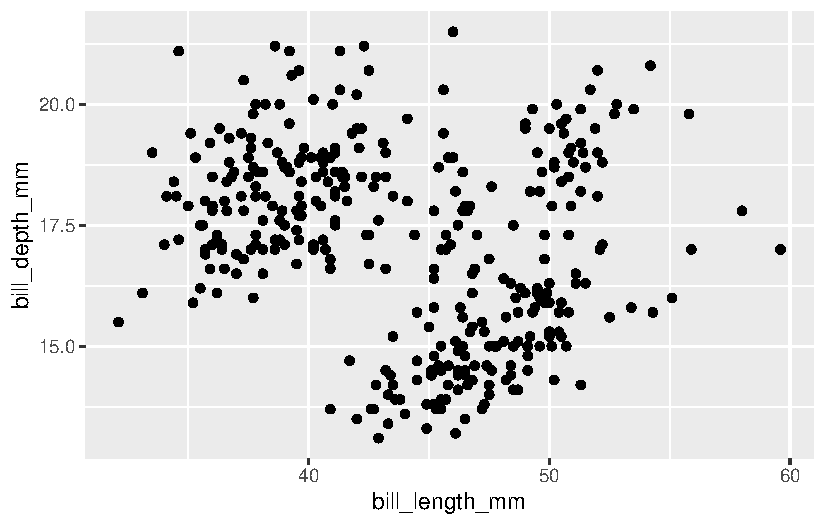
\includegraphics{basic_files/figure-pdf/unnamed-chunk-3-1.pdf}

\subsection{実行〇\textbar 出力〇\textbar コード×}

\textbf{チャンクでの書き方}

\begin{Shaded}
\begin{Highlighting}[]
\InformationTok{\textasciigrave{}\textasciigrave{}\textasciigrave{}\{r\}}
\InformationTok{\#| echo: false}

\InformationTok{1 + 1}


\InformationTok{ggplot(df) +}
\InformationTok{  geom\_point(aes(bill\_length\_mm, bill\_depth\_mm))}
\InformationTok{\textasciigrave{}\textasciigrave{}\textasciigrave{}}
\end{Highlighting}
\end{Shaded}

\textbf{コード表示}:なし

\begin{verbatim}
[1] 2
\end{verbatim}

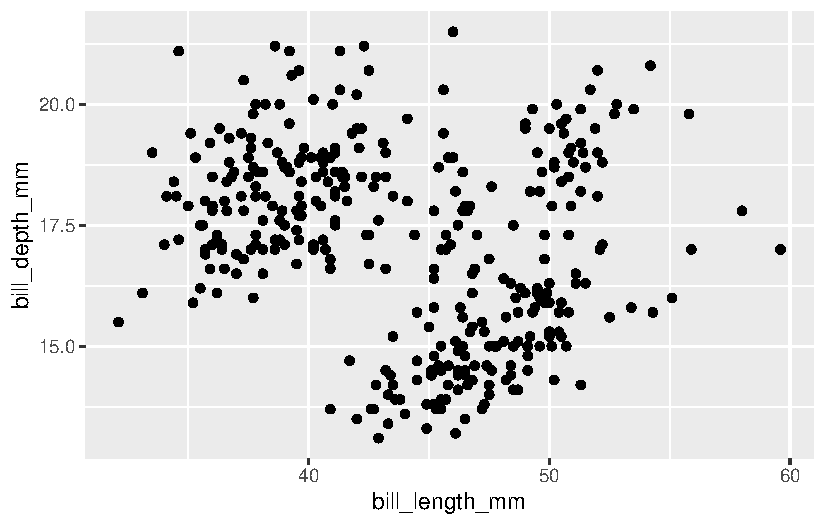
\includegraphics{basic_files/figure-pdf/unnamed-chunk-4-1.pdf}

\subsection{実行〇\textbar 出力×\textbar コード×}

\textbf{チャンクでの書き方}

\begin{Shaded}
\begin{Highlighting}[]
\InformationTok{\textasciigrave{}\textasciigrave{}\textasciigrave{}\{r\}}
\InformationTok{\#| include: false}

\InformationTok{1 + 1}


\InformationTok{ggplot(df) +}
\InformationTok{  geom\_point(aes(bill\_length\_mm, bill\_depth\_mm))}
\InformationTok{\textasciigrave{}\textasciigrave{}\textasciigrave{}}
\end{Highlighting}
\end{Shaded}

\textbf{コード表示}:なし

\subsection{実行〇\textbar 出力×(図はあり)\textbar コード〇}

\textbf{チャンクでの書き方}

\begin{Shaded}
\begin{Highlighting}[]
\InformationTok{\textasciigrave{}\textasciigrave{}\textasciigrave{}\{r\}}
\InformationTok{\#| results: hide}

\InformationTok{1 + 1}


\InformationTok{ggplot(df) +}
\InformationTok{  geom\_point(aes(bill\_length\_mm, bill\_depth\_mm))}
\InformationTok{\textasciigrave{}\textasciigrave{}\textasciigrave{}}
\end{Highlighting}
\end{Shaded}

\textbf{コード表示}

\begin{Shaded}
\begin{Highlighting}[]
\DecValTok{1} \SpecialCharTok{+} \DecValTok{1}


\FunctionTok{ggplot}\NormalTok{(df) }\SpecialCharTok{+}
  \FunctionTok{geom\_point}\NormalTok{(}\FunctionTok{aes}\NormalTok{(bill\_length\_mm, bill\_depth\_mm))}
\end{Highlighting}
\end{Shaded}

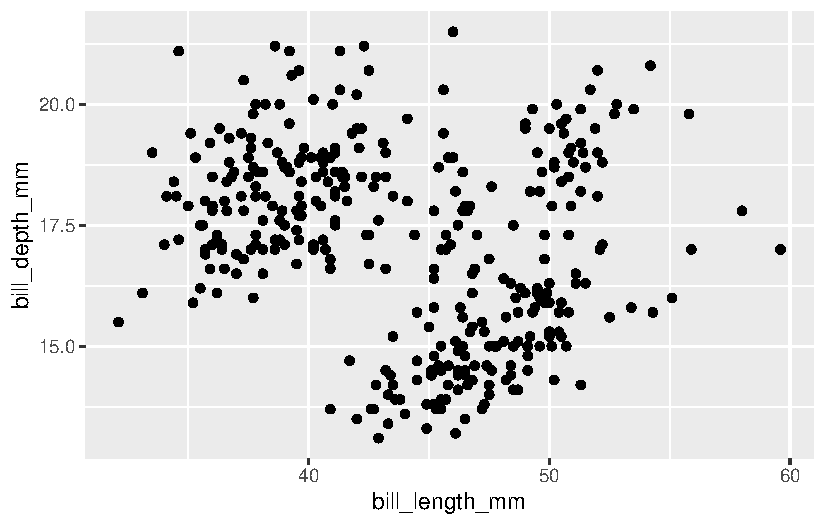
\includegraphics{basic_files/figure-pdf/unnamed-chunk-6-1.pdf}

\subsection{実行〇\textbar 出力×\textbar コード〇(1)}

\textbf{チャンクでの書き方}

\begin{Shaded}
\begin{Highlighting}[]
\InformationTok{\textasciigrave{}\textasciigrave{}\textasciigrave{}\{r\}}
\InformationTok{\#| results: hide}
\InformationTok{\#| fig{-}show: hide}

\InformationTok{1 + 1}


\InformationTok{ggplot(df) +}
\InformationTok{  geom\_point(aes(bill\_length\_mm, bill\_depth\_mm))}
\InformationTok{\textasciigrave{}\textasciigrave{}\textasciigrave{}}
\end{Highlighting}
\end{Shaded}

\textbf{コード表示}

\begin{Shaded}
\begin{Highlighting}[]
\DecValTok{1} \SpecialCharTok{+} \DecValTok{1}


\FunctionTok{ggplot}\NormalTok{(df) }\SpecialCharTok{+}
  \FunctionTok{geom\_point}\NormalTok{(}\FunctionTok{aes}\NormalTok{(bill\_length\_mm, bill\_depth\_mm))}
\end{Highlighting}
\end{Shaded}

\subsection{実行〇\textbar 出力×\textbar コード〇(2)}

\textbf{チャンクでの書き方}

\begin{Shaded}
\begin{Highlighting}[]
\InformationTok{\textasciigrave{}\textasciigrave{}\textasciigrave{}\{r\}}
\InformationTok{\#| output: false}

\InformationTok{1 + 1}


\InformationTok{ggplot(df) +}
\InformationTok{  geom\_point(aes(bill\_length\_mm, bill\_depth\_mm))}
\InformationTok{\textasciigrave{}\textasciigrave{}\textasciigrave{}}
\end{Highlighting}
\end{Shaded}

\textbf{コード表示}

\begin{Shaded}
\begin{Highlighting}[]
\DecValTok{1} \SpecialCharTok{+} \DecValTok{1}


\FunctionTok{ggplot}\NormalTok{(df) }\SpecialCharTok{+}
  \FunctionTok{geom\_point}\NormalTok{(}\FunctionTok{aes}\NormalTok{(bill\_length\_mm, bill\_depth\_mm))}
\end{Highlighting}
\end{Shaded}

\subsection{実行〇\textbar 出力×\textbar コード〇(チャンク)}

\begin{itemize}
\tightlist
\item
  公式ドキュメント\href{https://quarto.org/docs/computations/execution-options.html\#fenced-echo}{Fenced
  Echo}を参照
\end{itemize}

\textbf{チャンクでの書き方}

\begin{Shaded}
\begin{Highlighting}[]
\InformationTok{\textasciigrave{}\textasciigrave{}\textasciigrave{}\{r\}}
\InformationTok{\#| echo: fenced}

\InformationTok{1 + 1}


\InformationTok{ggplot(df) +}
\InformationTok{  geom\_point(aes(bill\_length\_mm, bill\_depth\_mm))}
\InformationTok{\textasciigrave{}\textasciigrave{}\textasciigrave{}}
\end{Highlighting}
\end{Shaded}

\textbf{チャンク表示}

\begin{Shaded}
\begin{Highlighting}[]
\InformationTok{\textasciigrave{}\textasciigrave{}\textasciigrave{}\{r\}}
\InformationTok{1 + 1}


\InformationTok{ggplot(df) +}
\InformationTok{  geom\_point(aes(bill\_length\_mm, bill\_depth\_mm))}
\InformationTok{\textasciigrave{}\textasciigrave{}\textasciigrave{}}
\end{Highlighting}
\end{Shaded}

\begin{verbatim}
[1] 2
\end{verbatim}

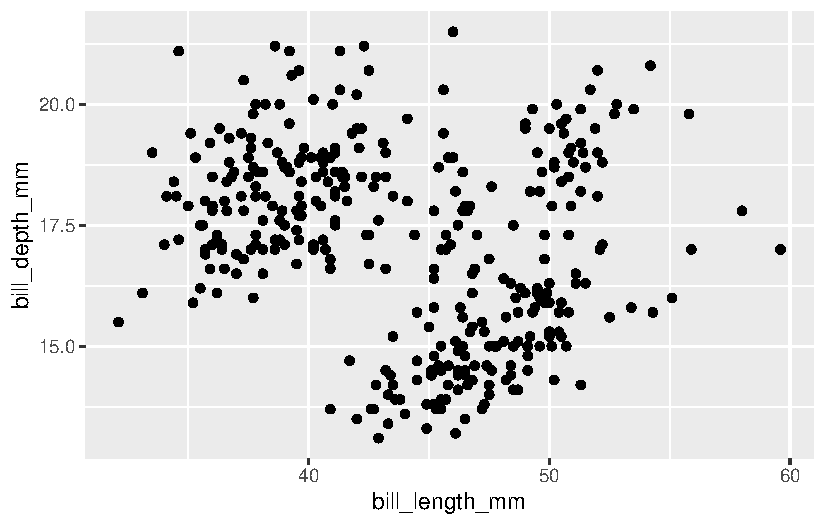
\includegraphics{basic_files/figure-pdf/unnamed-chunk-9-1.pdf}

\subsection{実行×\textbar 出力×\textbar コード〇}

\begin{itemize}
\tightlist
\item
  単にコードを表示したいだけの時に便利
\end{itemize}

\textbf{チャンクでの書き方}

\begin{Shaded}
\begin{Highlighting}[]
\InformationTok{\textasciigrave{}\textasciigrave{}\textasciigrave{}\{r\}}
\InformationTok{\#| echo: fenced}

\InformationTok{1 + 1}


\InformationTok{ggplot(df) +}
\InformationTok{  geom\_point(aes(bill\_length\_mm, bill\_depth\_mm))}
\InformationTok{\textasciigrave{}\textasciigrave{}\textasciigrave{}}
\end{Highlighting}
\end{Shaded}

\textbf{コード表示}

\begin{Shaded}
\begin{Highlighting}[]
\DecValTok{1} \SpecialCharTok{+} \DecValTok{1}


\FunctionTok{ggplot}\NormalTok{(df) }\SpecialCharTok{+}
  \FunctionTok{geom\_point}\NormalTok{(}\FunctionTok{aes}\NormalTok{(bill\_length\_mm, bill\_depth\_mm))}
\end{Highlighting}
\end{Shaded}

\subsection{実行×\textbar 出力×\textbar コード〇(チャンク)}

\begin{itemize}
\tightlist
\item
  \texttt{\{r\}}をさらに\texttt{\{\}}で囲んで\texttt{\{\{r\}\}}と2重に書く
\end{itemize}

\textbf{チャンクでの書き方}

\begin{Shaded}
\begin{Highlighting}[]
\InformationTok{\textasciigrave{}\textasciigrave{}\textasciigrave{}\{\{r\}\}}


\InformationTok{1 + 1}


\InformationTok{ggplot(df) +}
\InformationTok{  geom\_point(aes(bill\_length\_mm, bill\_depth\_mm))}
\InformationTok{\textasciigrave{}\textasciigrave{}\textasciigrave{}}
\end{Highlighting}
\end{Shaded}

\begin{itemize}
\tightlist
\item
  qmd上は上記書き方のみで「実行×\textbar 出力×\textbar コード〇(チャンク表示)」が実現できる

  \begin{itemize}
  \tightlist
  \item
    ただし解説目的で上記出力に\texttt{\{\{r\}\}}を表示させるためには,\texttt{\{\{\{r\}\}\}}と書く必要がある
  \item
    参照:\href{https://quarto.org/docs/computations/execution-options.html\#unexecuted-blocks}{Unexecuted
    Blocks};
    \href{https://quarto.org/docs/output-formats/html-code.html\#executable-blocks}{Executable
    Blocks}
  \end{itemize}
\end{itemize}

\textbf{チャンク表示}

\begin{Shaded}
\begin{Highlighting}[]
\InformationTok{\textasciigrave{}\textasciigrave{}\textasciigrave{}\{r\}}


\InformationTok{1 + 1}


\InformationTok{ggplot(df) +}
\InformationTok{  geom\_point(aes(bill\_length\_mm, bill\_depth\_mm))}
\InformationTok{\textasciigrave{}\textasciigrave{}\textasciigrave{}}
\end{Highlighting}
\end{Shaded}

\section{脚注}\label{ux811aux6ce8}

本文中に\texttt{{[}\^{}ここに数字や文字{]}}と書き,別途内容を記述することで,脚注(footnote)をつけることができる。

\begin{longtable}[]{@{}
  >{\raggedright\arraybackslash}p{(\columnwidth - 2\tabcolsep) * \real{0.4722}}
  >{\raggedright\arraybackslash}p{(\columnwidth - 2\tabcolsep) * \real{0.5278}}@{}}
\toprule\noalign{}
\begin{minipage}[b]{\linewidth}\raggedright
見え方
\end{minipage} & \begin{minipage}[b]{\linewidth}\raggedright
書き方
\end{minipage} \\
\midrule\noalign{}
\endhead
\bottomrule\noalign{}
\endlastfoot
基本の脚注\footnote{1行のみの脚注} & \texttt{基本の脚注{[}\^{}1{]}} \\
{[} {]}内は文字でもよい\footnote{文字でも脚注番号に変換される} &
\texttt{{[} {]}内は文字でもよい{[}\^{}word{]}} \\
脚注内容を本文中に\footnote{直接{[} {]}内に内容を書く} &
\texttt{脚注内容を本文中に\^{}{[}直接{[}\ {]}内に内容を書く{]}} \\
見え方と書き方で脚注番号が異なることも\footnote{これまでの脚注の文字数字とかぶらなければ自動で連番の数値に変換される}
& \texttt{見え方と書き方で脚注番号が異なることも{[}\^{}2{]}} \\
脚注を複数行に分ける\footnote{複数行書くためにインデントで区別する。以下1行ずつ空ける必要あり

  2段落目

  3段落目

  4段落目} & \texttt{脚注を複数行に分ける{[}\^{}multiple{]}} \\
\end{longtable}

脚注内容

\begin{verbatim}
[^1]: 脚注の内容を本文とは別に書く
[^word]:文字でも脚注番号に変換される 
[^2]: これまでの脚注の文字数字とかぶらなければ自動で連番の数値に変換される
[^multiple]: 複数行書くためにインデントで区別する。以下1行ずつ空ける必要あり。

      2段落目
      
      3段落目
      
      4段落目  


【補足】
本来は[^multiple]で以下のように書きたかったが,pdfでエラーになるので省略

> { }でコードも書ける 

>    { 1+1 }
\end{verbatim}

ここが脚注の記述内容

\section{セクションへのリンク}\label{ux30bbux30afux30b7ux30e7ux30f3ux3078ux306eux30eaux30f3ux30af}

\begin{longtable}[]{@{}ll@{}}
\toprule\noalign{}
見え方 & 書き方 \\
\midrule\noalign{}
\endhead
\bottomrule\noalign{}
\endlastfoot
Chapter~\ref{sec-caution} & \texttt{{[}@sec-caution{]}} \\
\ref{sec-caution} & \texttt{{[}-@sec-caution{]}} \\
セクション~\ref{sec-caution} &
\texttt{{[}セクション\ -@sec-caution{]}} \\
\ref{sec-caution}章 & \texttt{{[}-@sec-caution{]}章} \\
\ref{sec-caution} & \texttt{{[}-@sec-caution\ 章{]}} \\
\hyperref[sec-caution]{注意事項} &
\texttt{{[}注意事項{]}(\#sec-caution)} \\
& \\
& \\
\end{longtable}

\section{図表へのリンク}\label{ux56f3ux8868ux3078ux306eux30eaux30f3ux30af}

\begin{longtable}[]{@{}ll@{}}
\toprule\noalign{}
見え方 & 書き方 \\
\midrule\noalign{}
\endhead
\bottomrule\noalign{}
\endlastfoot
Figure~\ref{fig-zu} を参照 & \texttt{@fig-zu\ を参照} \\
図~\ref{fig-zu} を参照 & \texttt{{[}図\ -@fig-zu{]}\ を参照} \\
Table~\ref{tbl-hyo} を参照 & \texttt{@tbl-hyo\ を参照} \\
表~\ref{tbl-hyo}を参照 & \texttt{{[}表\ -@tbl-hyo{]}を参照} \\
\end{longtable}

\section{コールアウト}\label{ux30b3ux30fcux30ebux30a2ux30a6ux30c8}

\begin{itemize}
\tightlist
\item
  公式ドキュメントの参照箇所

  \begin{itemize}
  \tightlist
  \item
    \href{https://quarto.org/docs/authoring/callouts.html}{Callout
    Blocks}
  \end{itemize}
\end{itemize}

\subsection{基本の型}\label{ux57faux672cux306eux578b}

\begin{Shaded}
\begin{Highlighting}[]
\NormalTok{::: \{.callout{-}note\}}
\NormalTok{ここにテキスト}
\NormalTok{:::}
\end{Highlighting}
\end{Shaded}

\begin{tcolorbox}[enhanced jigsaw, bottomtitle=1mm, toptitle=1mm, title=\textcolor{quarto-callout-note-color}{\faInfo}\hspace{0.5em}{Note}, breakable, arc=.35mm, opacitybacktitle=0.6, leftrule=.75mm, rightrule=.15mm, colframe=quarto-callout-note-color-frame, colback=white, colbacktitle=quarto-callout-note-color!10!white, toprule=.15mm, coltitle=black, left=2mm, titlerule=0mm, bottomrule=.15mm, opacityback=0]

ここにテキスト

\end{tcolorbox}

\begin{Shaded}
\begin{Highlighting}[]
\NormalTok{::: \{.callout{-}tip\}}
\NormalTok{ここにテキスト}
\NormalTok{:::}
\end{Highlighting}
\end{Shaded}

\begin{tcolorbox}[enhanced jigsaw, bottomtitle=1mm, toptitle=1mm, title=\textcolor{quarto-callout-tip-color}{\faLightbulb}\hspace{0.5em}{Tip}, breakable, arc=.35mm, opacitybacktitle=0.6, leftrule=.75mm, rightrule=.15mm, colframe=quarto-callout-tip-color-frame, colback=white, colbacktitle=quarto-callout-tip-color!10!white, toprule=.15mm, coltitle=black, left=2mm, titlerule=0mm, bottomrule=.15mm, opacityback=0]

ここにテキスト

\end{tcolorbox}

\begin{Shaded}
\begin{Highlighting}[]
\NormalTok{::: \{.callout{-}warning\}}
\NormalTok{ここにテキスト}
\NormalTok{:::}
\end{Highlighting}
\end{Shaded}

\begin{tcolorbox}[enhanced jigsaw, bottomtitle=1mm, toptitle=1mm, title=\textcolor{quarto-callout-warning-color}{\faExclamationTriangle}\hspace{0.5em}{Warning}, breakable, arc=.35mm, opacitybacktitle=0.6, leftrule=.75mm, rightrule=.15mm, colframe=quarto-callout-warning-color-frame, colback=white, colbacktitle=quarto-callout-warning-color!10!white, toprule=.15mm, coltitle=black, left=2mm, titlerule=0mm, bottomrule=.15mm, opacityback=0]

ここにテキスト

\end{tcolorbox}

\begin{Shaded}
\begin{Highlighting}[]
\NormalTok{::: \{.callout{-}caution\}}
\NormalTok{ここにテキスト}
\NormalTok{:::}
\end{Highlighting}
\end{Shaded}

\begin{tcolorbox}[enhanced jigsaw, bottomtitle=1mm, toptitle=1mm, title=\textcolor{quarto-callout-caution-color}{\faFire}\hspace{0.5em}{Caution}, breakable, arc=.35mm, opacitybacktitle=0.6, leftrule=.75mm, rightrule=.15mm, colframe=quarto-callout-caution-color-frame, colback=white, colbacktitle=quarto-callout-caution-color!10!white, toprule=.15mm, coltitle=black, left=2mm, titlerule=0mm, bottomrule=.15mm, opacityback=0]

ここにテキスト

\end{tcolorbox}

\begin{Shaded}
\begin{Highlighting}[]
\NormalTok{::: \{.callout{-}important\}}
\NormalTok{ここにテキスト}
\NormalTok{:::}
\end{Highlighting}
\end{Shaded}

\begin{tcolorbox}[enhanced jigsaw, bottomtitle=1mm, toptitle=1mm, title=\textcolor{quarto-callout-important-color}{\faExclamation}\hspace{0.5em}{Important}, breakable, arc=.35mm, opacitybacktitle=0.6, leftrule=.75mm, rightrule=.15mm, colframe=quarto-callout-important-color-frame, colback=white, colbacktitle=quarto-callout-important-color!10!white, toprule=.15mm, coltitle=black, left=2mm, titlerule=0mm, bottomrule=.15mm, opacityback=0]

ここにテキスト

\end{tcolorbox}

\subsection{見え方の変更}\label{ux898bux3048ux65b9ux306eux5909ux66f4}

\textbf{書き方}

\begin{Shaded}
\begin{Highlighting}[]
\NormalTok{::: \{.callout{-}note\}}
\FunctionTok{\#\#\#\# メモ}
\NormalTok{タイトルを変更}
\NormalTok{:::}
\end{Highlighting}
\end{Shaded}

\textbf{出力}

\begin{tcolorbox}[enhanced jigsaw, bottomtitle=1mm, toptitle=1mm, title=\textcolor{quarto-callout-note-color}{\faInfo}\hspace{0.5em}{メモ}, breakable, arc=.35mm, opacitybacktitle=0.6, leftrule=.75mm, rightrule=.15mm, colframe=quarto-callout-note-color-frame, colback=white, colbacktitle=quarto-callout-note-color!10!white, toprule=.15mm, coltitle=black, left=2mm, titlerule=0mm, bottomrule=.15mm, opacityback=0]

タイトルを変更

\end{tcolorbox}

\textbf{書き方}

\begin{Shaded}
\begin{Highlighting}[]
\NormalTok{::: \{.callout{-}note collapse="true"\}}
\FunctionTok{\#\#\#\# 折りたたみもできる}
\NormalTok{ここにテキスト}
\NormalTok{:::}
\end{Highlighting}
\end{Shaded}

\textbf{出力}

\begin{tcolorbox}[enhanced jigsaw, bottomtitle=1mm, toptitle=1mm, title=\textcolor{quarto-callout-note-color}{\faInfo}\hspace{0.5em}{折りたたみもできる}, breakable, arc=.35mm, opacitybacktitle=0.6, leftrule=.75mm, rightrule=.15mm, colframe=quarto-callout-note-color-frame, colback=white, colbacktitle=quarto-callout-note-color!10!white, toprule=.15mm, coltitle=black, left=2mm, titlerule=0mm, bottomrule=.15mm, opacityback=0]

ここにテキスト

\end{tcolorbox}

\textbf{書き方}

\begin{Shaded}
\begin{Highlighting}[]
\NormalTok{::: \{.callout{-}note\}}
\FunctionTok{\#\#\#\# メモ}
\NormalTok{アイコンなし}
\NormalTok{:::}
\end{Highlighting}
\end{Shaded}

\textbf{出力}

\begin{tcolorbox}[enhanced jigsaw, bottomtitle=1mm, toptitle=1mm, title={メモ}, breakable, arc=.35mm, opacitybacktitle=0.6, leftrule=.75mm, rightrule=.15mm, colframe=quarto-callout-note-color-frame, colback=white, colbacktitle=quarto-callout-note-color!10!white, toprule=.15mm, coltitle=black, left=2mm, titlerule=0mm, bottomrule=.15mm, opacityback=0]

アイコンなし

\end{tcolorbox}

\textbf{書き方}

\begin{Shaded}
\begin{Highlighting}[]
\NormalTok{::: \{.callout{-}note appearance="simple"\}}
\FunctionTok{\#\#\#\# シンプルに}
\NormalTok{ここにテキスト}
\NormalTok{:::}
\end{Highlighting}
\end{Shaded}

\textbf{出力}

\begin{tcolorbox}[enhanced jigsaw, colframe=quarto-callout-note-color-frame, colback=white, toprule=.15mm, opacityback=0, breakable, arc=.35mm, bottomrule=.15mm, leftrule=.75mm, rightrule=.15mm, left=2mm]
\begin{minipage}[t]{5.5mm}
\textcolor{quarto-callout-note-color}{\faInfo}
\end{minipage}%
\begin{minipage}[t]{\textwidth - 5.5mm}

\vspace{-3mm}\textbf{シンプルに}\vspace{3mm}

ここにテキスト

\end{minipage}%
\end{tcolorbox}

\textbf{書き方}

\begin{Shaded}
\begin{Highlighting}[]
\NormalTok{::: \{.callout{-}note appearance="minimal"\}}
\FunctionTok{\#\#\#\# シンプルでアイコンなし}
\NormalTok{ここにテキスト}
\NormalTok{:::}
\end{Highlighting}
\end{Shaded}

\textbf{出力}

\begin{tcolorbox}[enhanced jigsaw, colframe=quarto-callout-note-color-frame, colback=white, toprule=.15mm, opacityback=0, breakable, arc=.35mm, bottomrule=.15mm, leftrule=.75mm, rightrule=.15mm, left=2mm]

\vspace{-3mm}\textbf{シンプルでアイコンなし}\vspace{3mm}

ここにテキスト

\end{tcolorbox}

\subsection{コールアウトへのリンク}\label{ux30b3ux30fcux30ebux30a2ux30a6ux30c8ux3078ux306eux30eaux30f3ux30af}

\begin{tcolorbox}[enhanced jigsaw, bottomtitle=1mm, toptitle=1mm, title=\textcolor{quarto-callout-note-color}{\faInfo}\hspace{0.5em}{Note \ref*{nte-example} }, breakable, arc=.35mm, opacitybacktitle=0.6, leftrule=.75mm, rightrule=.15mm, colframe=quarto-callout-note-color-frame, colback=white, colbacktitle=quarto-callout-note-color!10!white, toprule=.15mm, coltitle=black, left=2mm, titlerule=0mm, bottomrule=.15mm, opacityback=0]

\quartocalloutnte{nte-example} 

ここにテキスト

\end{tcolorbox}

Note~\ref{nte-example} を参照

https://quarto.org/docs/authoring/callouts.html\#tbl-callout-prefixes

\section{MacのPCのキーボード記号の意味}\label{macux306epcux306eux30adux30fcux30dcux30fcux30c9ux8a18ux53f7ux306eux610fux5473}

\begin{itemize}
\item
  Quartoの公式ドキュメントでは,当たり前のように使われているので,知らないと読み解けない
\item
  Apple公式の説明

  \begin{itemize}
  \tightlist
  \item
    \href{https://support.apple.com/ja-jp/guide/mac-help/cpmh0011/mac}{Macのメニューに表示される記号}
  \item
    \href{https://support.apple.com/ja-jp/HT201236}{Mac
    のキーボードショートカット} (記号がコピペできる)
  \end{itemize}
\end{itemize}

\begin{longtable}[]{@{}ll@{}}
\toprule\noalign{}
意味 & 記号 \\
\midrule\noalign{}
\endhead
\bottomrule\noalign{}
\endlastfoot
Commandキー & ⌘ \\
Shiftキー & ⇧ \\
Optionキー & ⌥ \\
Controlキー & ⌃ \\
\end{longtable}

\bookmarksetup{startatroot}

\chapter{図表}\label{sec-caution}

\section{図}\label{ux56f3}

\begin{Shaded}
\begin{Highlighting}[]
\InformationTok{\textasciigrave{}\textasciigrave{}\textasciigrave{}\{r\}}
\InformationTok{\#| label: fig{-}zu}
\InformationTok{\#| fig{-}cap: "散布図"}

\InformationTok{library(ggplot2)}
\InformationTok{ggplot(mtcars) +}
\InformationTok{  geom\_point(aes(mpg,disp))}
\InformationTok{\textasciigrave{}\textasciigrave{}\textasciigrave{}}
\end{Highlighting}
\end{Shaded}

\begin{figure}[H]

\centering{

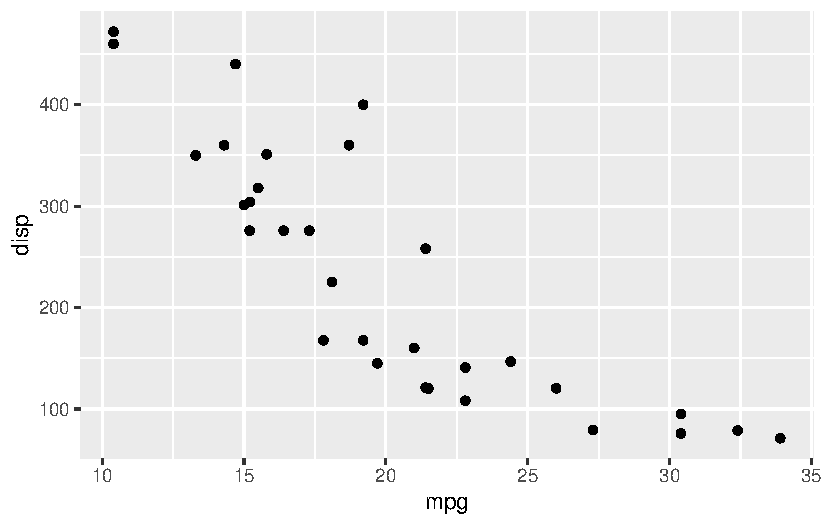
\includegraphics{fig_table_files/figure-pdf/fig-zu-1.pdf}

}

\caption{\label{fig-zu}散布図}

\end{figure}%

Figure~\ref{fig-zu} を参照

\section{表}\label{ux8868}

\begin{longtable}[]{@{}lll@{}}
\caption{表タイトル}\label{tbl-hyo}\tabularnewline
\toprule\noalign{}
Col1 & Col2 & Col3 \\
\midrule\noalign{}
\endfirsthead
\toprule\noalign{}
Col1 & Col2 & Col3 \\
\midrule\noalign{}
\endhead
\bottomrule\noalign{}
\endlastfoot
x & 1 & 10 \\
y & 0 & 20 \\
\end{longtable}

Table~\ref{tbl-hyo} を参照

\bookmarksetup{startatroot}

\chapter{注意事項}\label{sec-caution}

\begin{itemize}
\tightlist
\item
  奇数ページだと1ページ白紙になるので,偶数ページにしないとだめ
\item
  前半,後半部分は,PDFとして作成するときはページ数増えるので不要かも
\end{itemize}

\bookmarksetup{startatroot}

\chapter{引用文献の書き方}\label{sec-sanko}

\section{引用文献の書き方}\label{ux5f15ux7528ux6587ux732eux306eux66f8ux304dux65b9}

まずプロジェクトフォルダ内に\texttt{references.bib}ファイルを作成する。自ら記入していくこともできるが,引用する文献を\href{https://scholar.google.com/}{Google
Scholar}で検索し Figure~\ref{fig-gscholar}
,BibTeX形式で表示してコピーし Figure~\ref{fig-gscholar-cite}
,ファイル内にペーストしていくと簡単である。

\begin{figure}

\centering{


\includegraphics[width=6.35417in,height=\textheight]{images/google-scholar.png}

}

\caption{\label{fig-gscholar}文献を表示して引用をクリックする}

\end{figure}%

\begin{figure}

\centering{


\includegraphics[width=5.02083in,height=\textheight]{images/google-scholar-cite.png}

}

\caption{\label{fig-gscholar-cite}BibTeXをクリックする}

\end{figure}%

次にYAMLヘッダー内に,つまりBooksの時は\texttt{\_quarto.yml}内に,以下を書く

\begin{Shaded}
\begin{Highlighting}[]
\PreprocessorTok{{-}{-}{-}}
\FunctionTok{bibliography}\KeywordTok{:}\AttributeTok{ references.bib}
\PreprocessorTok{{-}{-}{-}}
\end{Highlighting}
\end{Shaded}

文献を引用したい箇所に以下のように記述する。

\begin{Shaded}
\begin{Highlighting}[]
\NormalTok{引用文献はこちら}\CommentTok{[}\OtherTok{@wickham2023r;@wickham2019welcome}\CommentTok{]}  
\NormalTok{Wickham}\CommentTok{[}\OtherTok{@wickham2023r}\CommentTok{]}\NormalTok{は述べた  }
\NormalTok{@wickham2023r は述べた  }
\end{Highlighting}
\end{Shaded}

\textbf{出力例}

引用文献はこちら (Wickham, Çetinkaya-Rundel, and Grolemund 2023; Wickham
et al. 2019)\\
Wickham (Wickham, Çetinkaya-Rundel, and Grolemund 2023)は述べた\\
Wickham, Çetinkaya-Rundel, and Grolemund (2023) は述べた

本文中の文献表示の形式を変えたい場合は,YAMLヘッダー内に\texttt{csl:対応するcslファイル}を追記する

\begin{Shaded}
\begin{Highlighting}[]
\PreprocessorTok{{-}{-}{-}}
\FunctionTok{bibliography}\KeywordTok{:}\AttributeTok{ references.bib}
\FunctionTok{csl}\KeywordTok{:}\AttributeTok{ nature.csl}
\PreprocessorTok{{-}{-}{-}}
\end{Highlighting}
\end{Shaded}

入手先:\href{https://github.com/citation-style-language/styles/blob/master/nature.csl}{nature.csl}

\textbf{出力例}

\begin{quote}
引用文献はこちら\textsuperscript{1,2}\\
wickham\textsuperscript{1}は述べた\\
\textsuperscript{1} は述べた
\end{quote}

文献リストは,何も指定しなければ引用した箇所のセクションの最下部に作られる。巻末に作成したい場合は,引用文献のセクションを作り,そこに以下のように記述する。

\begin{Shaded}
\begin{Highlighting}[]
\FunctionTok{\#\# 引用文献}

\NormalTok{:::\{\#refs\}}

\NormalTok{:::}
\end{Highlighting}
\end{Shaded}

\bookmarksetup{startatroot}

\chapter*{引用文献}\label{ux5f15ux7528ux6587ux732e}
\addcontentsline{toc}{chapter}{引用文献}

\markboth{引用文献}{引用文献}

\phantomsection\label{refs}
\begin{CSLReferences}{1}{0}
\bibitem[\citeproctext]{ref-wickham2019welcome}
Wickham, Hadley, Mara Averick, Jennifer Bryan, Winston Chang, Lucy
D'Agostino McGowan, Romain François, Garrett Grolemund, et al. 2019.
{``Welcome to the Tidyverse.''} \emph{Journal of Open Source Software} 4
(43): 1686.

\bibitem[\citeproctext]{ref-wickham2023r}
Wickham, Hadley, Mine Çetinkaya-Rundel, and Garrett Grolemund. 2023.
\emph{R for Data Science}. " O'Reilly Media, Inc.".

\end{CSLReferences}



\clearpage
\vspace*{\stretch{1}}
\begin{flushright}
\begin{minipage}{0.5\hsize}
\begin{description}
  \item{著者:} 著者名
  \item{発行:} 2019年11月18日
  \item{サークル名:} サークル名
  \item{連絡先:} メールアドレス
  \item{印刷:} 印刷所名
\end{description}
\end{minipage}
\end{flushright}
\clearpage

\end{document}
